\subsection{Case Study 2: Apache Cassandra}
\vspace{10pt}

\mm{
Apache Cassandra is a Table/Key-Value hybrid NoSQL database.  It is suitable for applications that require high availability provided by replication.  In terms of the CAP theorem, Cassandra prioritizes availability and performance over consistency, making it highly performant and scalable, though consistency is eventual rather than strong, for typical Cassandra applications.
 
Apache Cassandra was installed on Amazon EC2 instances of various VM instance types.  Our testing was done on Cassandra clusters with 5 nodes.  We ran our testing with a replication factor of three, so every database record was stored on three of the five nodes.  We tested using weak (or eventual) consistency, using a consistency level of "ONE".

We ran the YCSB client on a m4.2xlarge EC2 instance running Ubuntu Linux 14.04. We monitored the system load average on the client machine to verify that the client was not the bottleneck during the tests.
}

\begin{comment}
  \begin{figure}
  \centering
    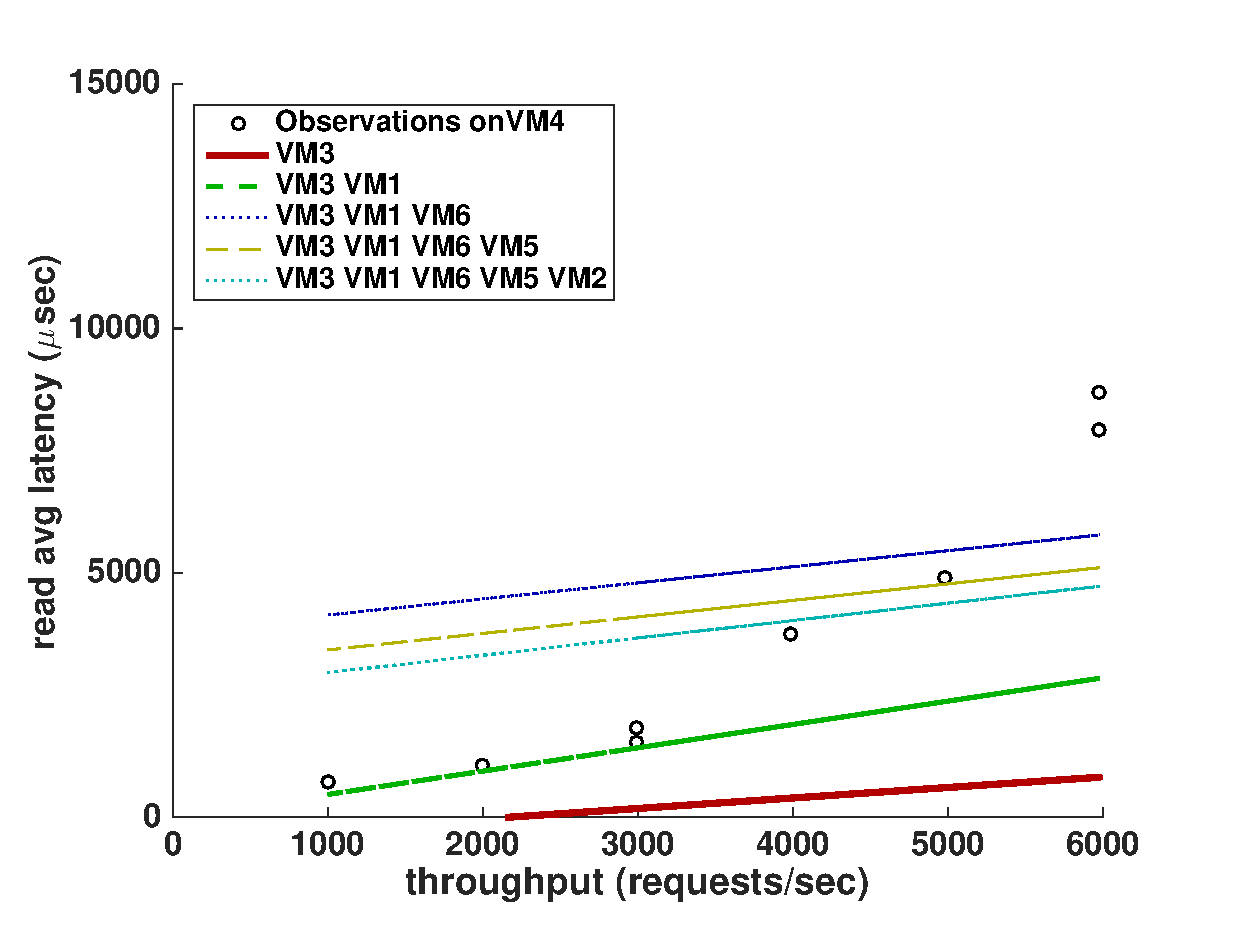
\includegraphics[scale = 0.25]{cassandra_fit_read_avg_latency_m3_2x_m3__r3_2x_r3_x_m3_x_r3_.eps}
    \caption{Cassandra average read latency vs throughput}
    \label{figure:redisbarread}
  \end{figure}

  \begin{figure}
  \centering
    \includegraphics[scale = 0.25]{cassandra_fit_read_avg_latency_r3_2x_r3_x_m3_x_m3__m3_2x_r3_.eps}
    \caption{Cassandra average read latency vs throughput}
    \label{figure:redisbarread}
  \end{figure}

  \begin{figure}
  \centering
    \includegraphics[scale = 0.25]{cassandra_fit_read_avg_latency_r3__m3_x_r3_2x_m3_2x_r3_x_m3_.eps}
    \caption{Cassandra average read latency vs throughput}
    \label{figure:redisbarread}
  \end{figure}

  \begin{figure}
  \centering
    \includegraphics[scale = 0.25]{cassandra_fit_read_avg_latency_r3_x_m3__r3_2x_m3_x_m3_2x_r3_.eps}
    \caption{Cassandra average read latency vs throughput}
    \label{figure:redisbarread}
  \end{figure}
\end{comment}

\begin{figure*}[t]
\subfloat[fig 1]{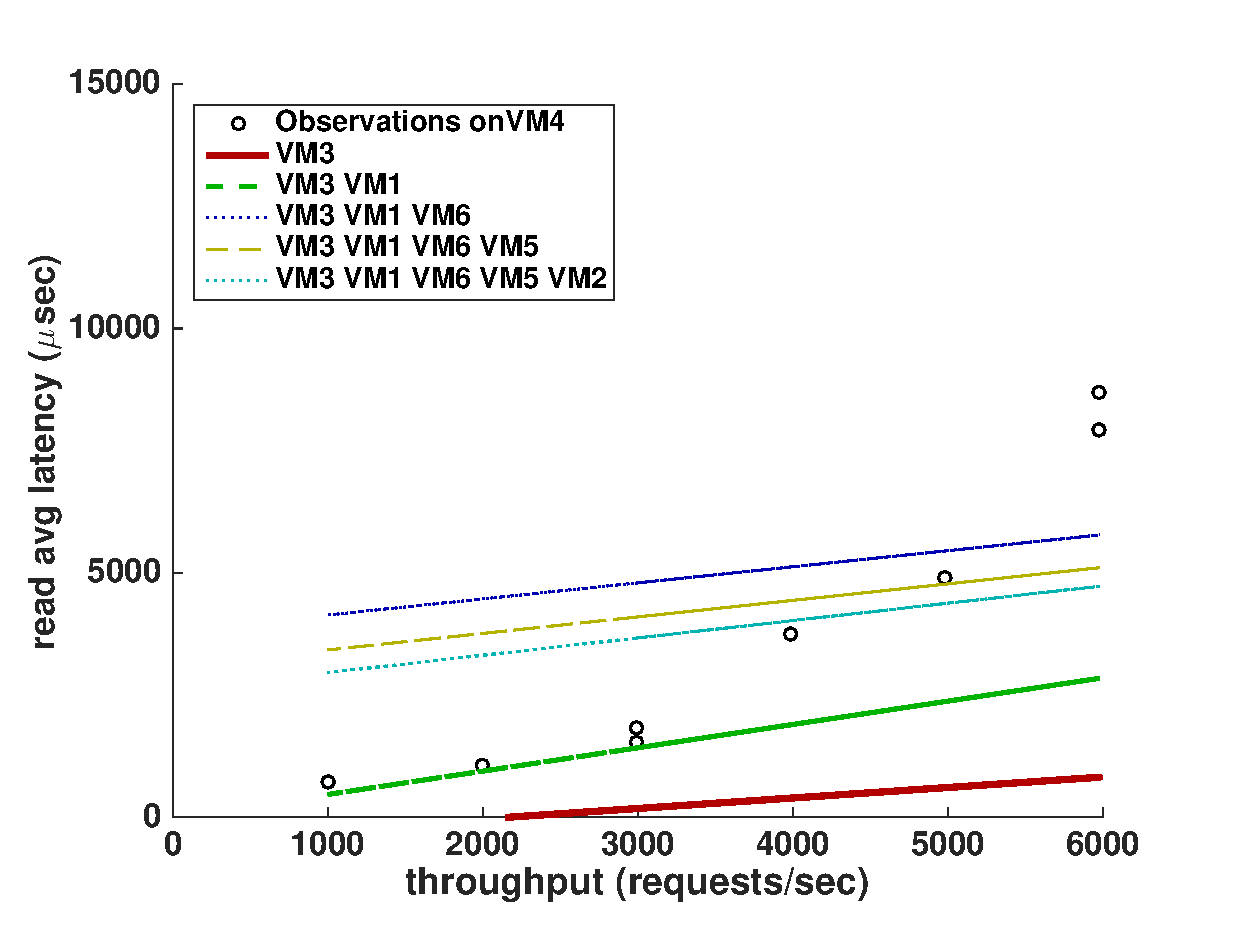
\includegraphics[width=0.5\textwidth]{cassandra_fit_read_avg_latency_m3_2x_m3__r3_2x_r3_x_m3_x_r3_.eps}} 
\subfloat[fig 2]{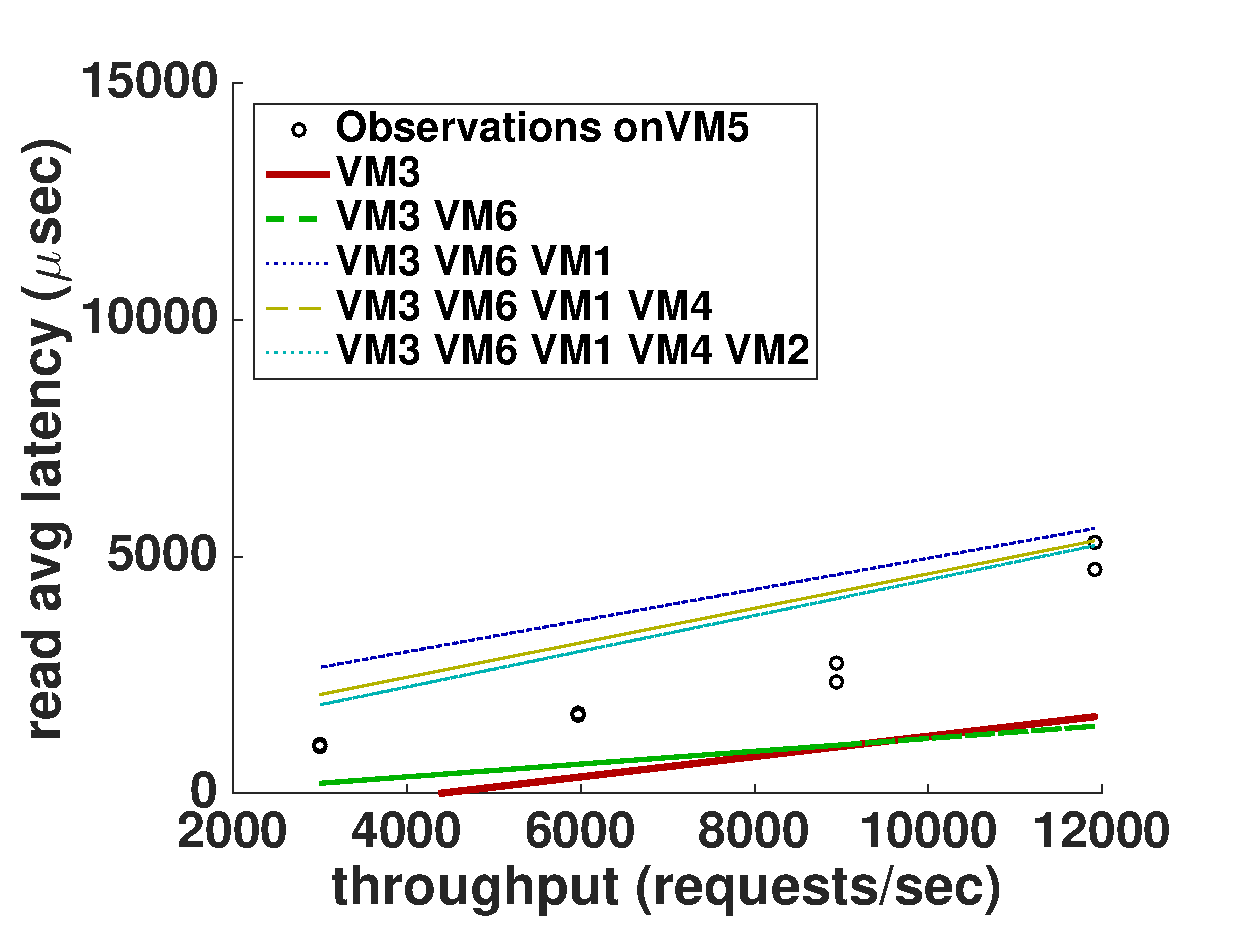
\includegraphics[width=0.5\textwidth]{cassandra_fit_read_avg_latency_m3_2x_r3_2x_m3__r3__m3_x_r3_x.eps}}\\
\subfloat[fig 3]{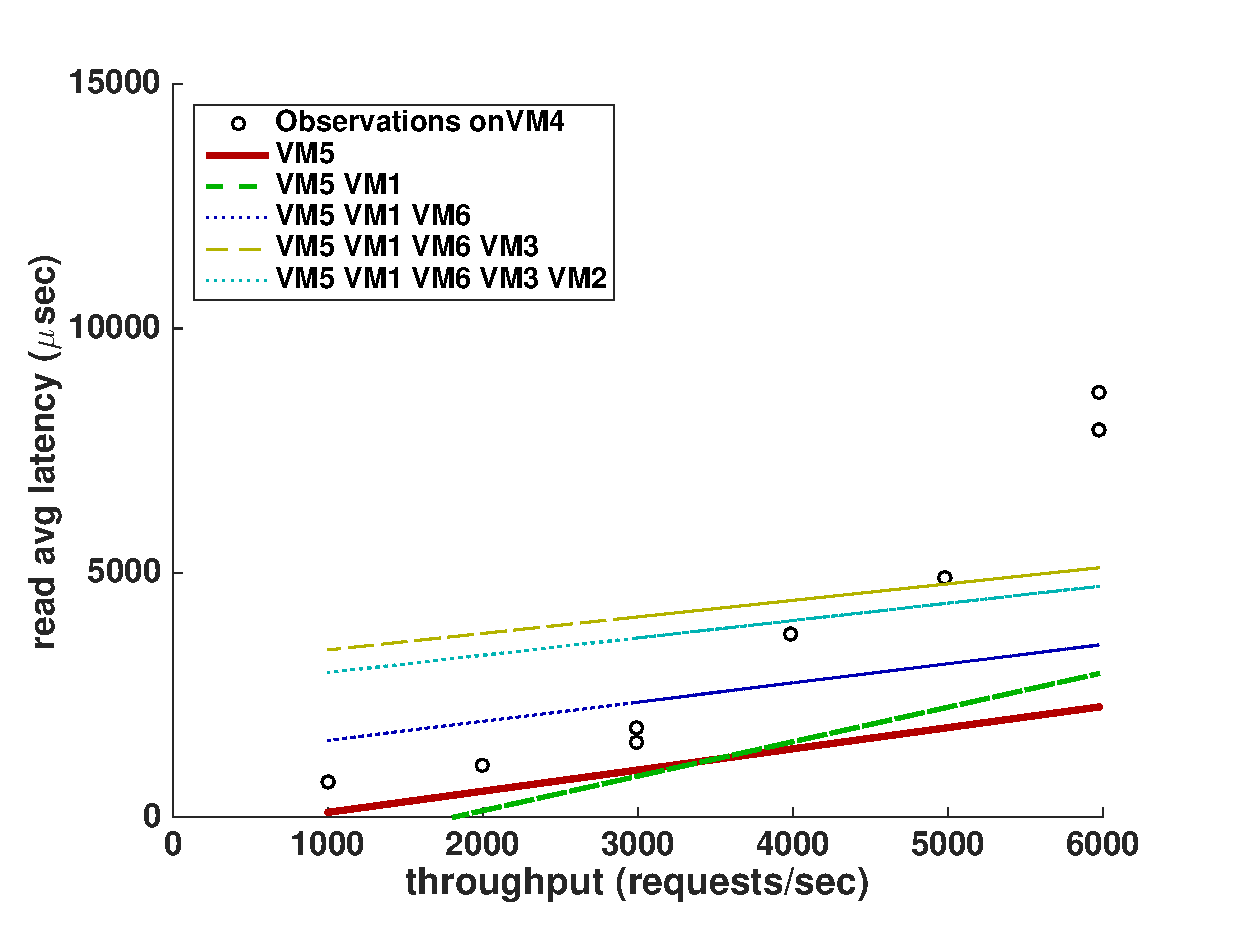
\includegraphics[width=0.5\textwidth]{cassandra_fit_read_avg_latency_r3_x_m3__r3_2x_m3_2x_m3_x_r3_.eps}}
\subfloat[fig 4]{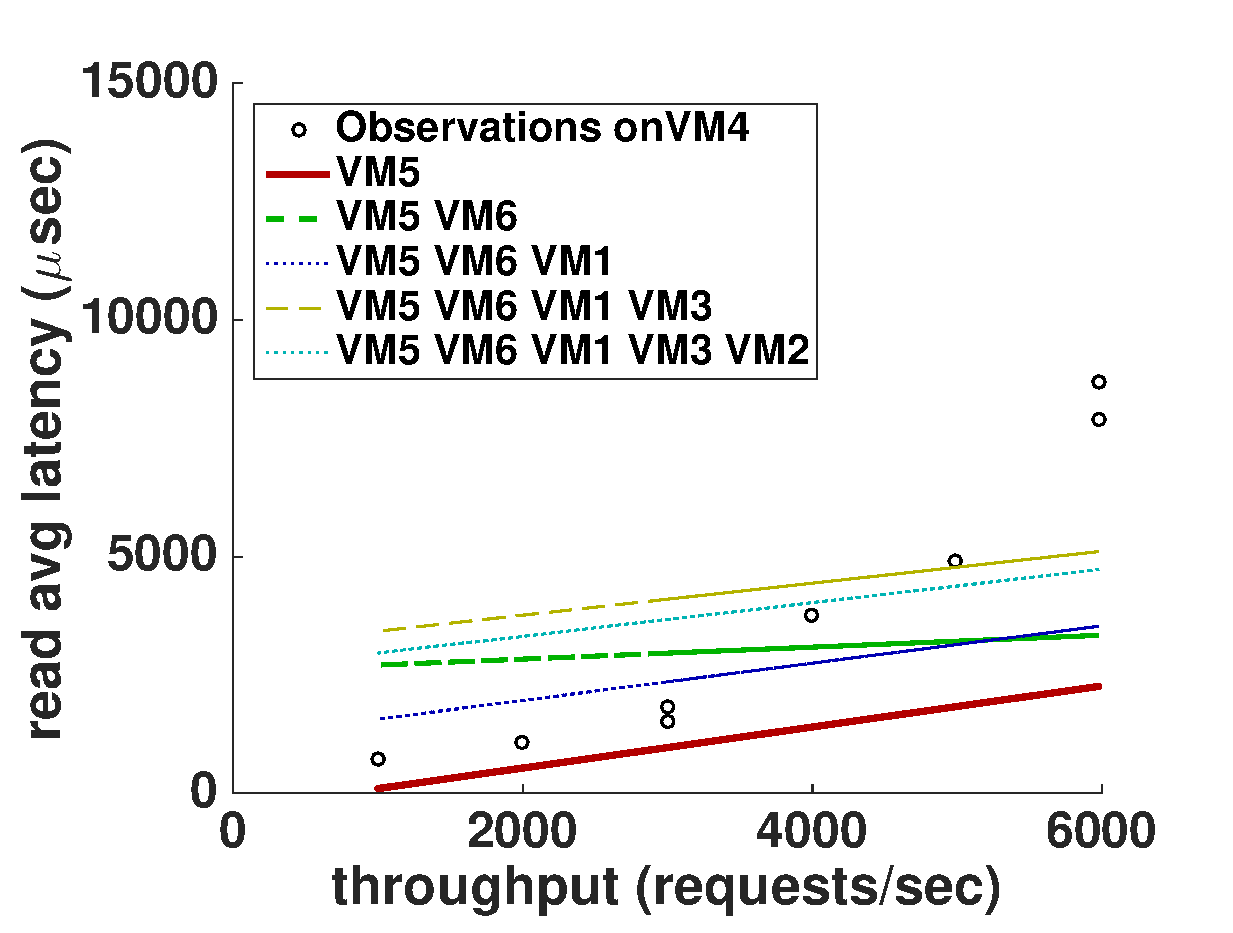
\includegraphics[width=0.5\textwidth]{cassandra_fit_read_avg_latency_r3_x_r3_2x_m3__m3_2x_m3_x_r3_.eps}}
\caption{Incremental fit for Cassandra Average Read Latency }
\label{some example}
\end{figure*}

\begin{comment}
  \begin{figure}
  \centering
    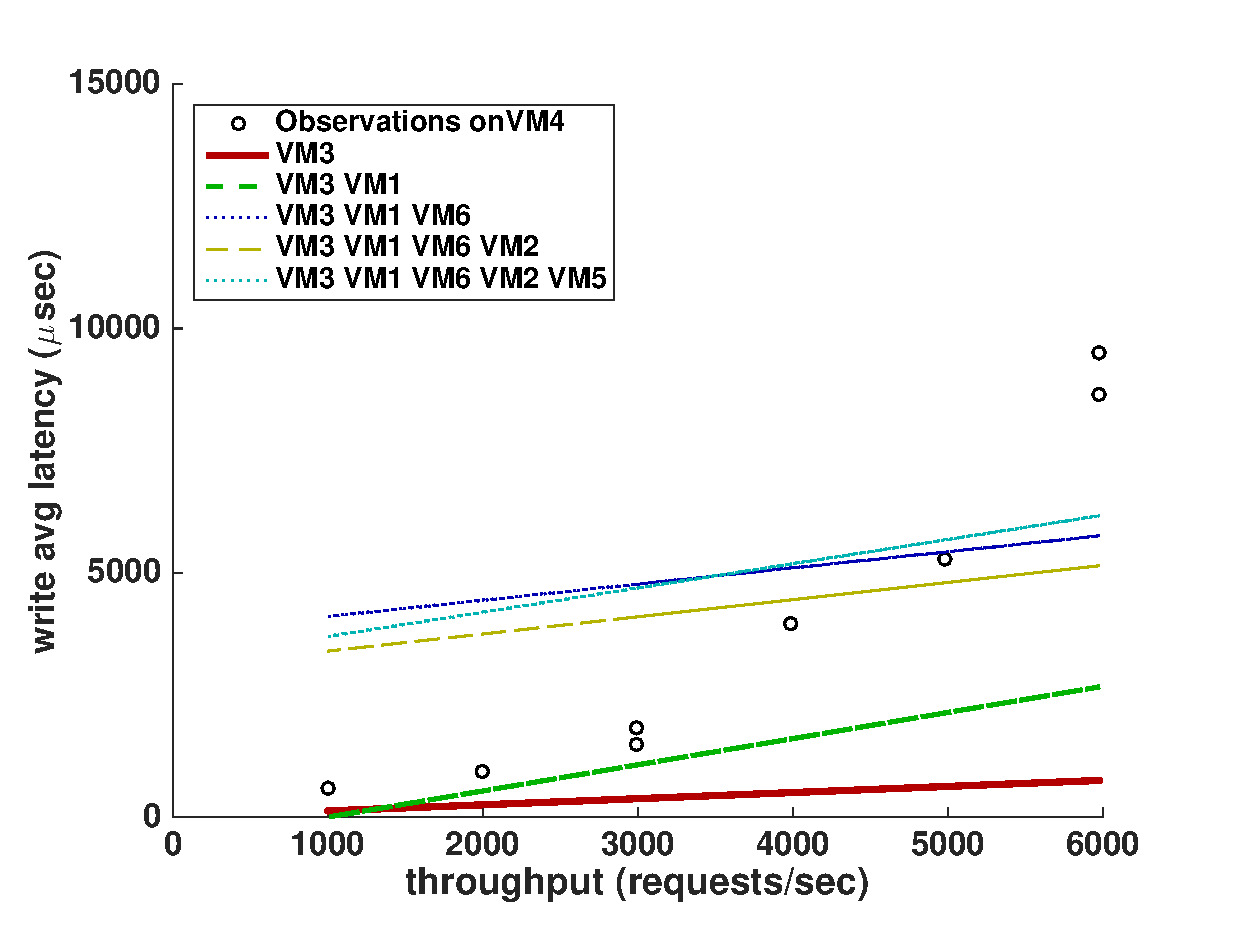
\includegraphics[scale = 0.25]{cassandra_fit_write_avg_latency_m3_2x_m3__r3_2x_m3_x_r3_x_r3_.eps}
    \caption{Cassandra average read latency vs throughput}
    \label{figure:redisbarread}
  \end{figure}

  \begin{figure}
  \centering
    \includegraphics[scale = 0.25]{cassandra_fit_write_avg_latency_m3_2x_m3_x_r3__r3_2x_r3_x_m3_.eps}
    \caption{Cassandra average read latency vs throughput}
    \label{figure:redisbarread}
  \end{figure}

  \begin{figure}
  \centering
    \includegraphics[scale = 0.25]{cassandra_fit_write_avg_latency_m3_2x_r3_x_r3_2x_m3_x_r3__m3_.eps}
    \caption{Cassandra average write latency vs throughput}
    \label{figure:redisbarread}
  \end{figure}

  \begin{figure}
  \centering
    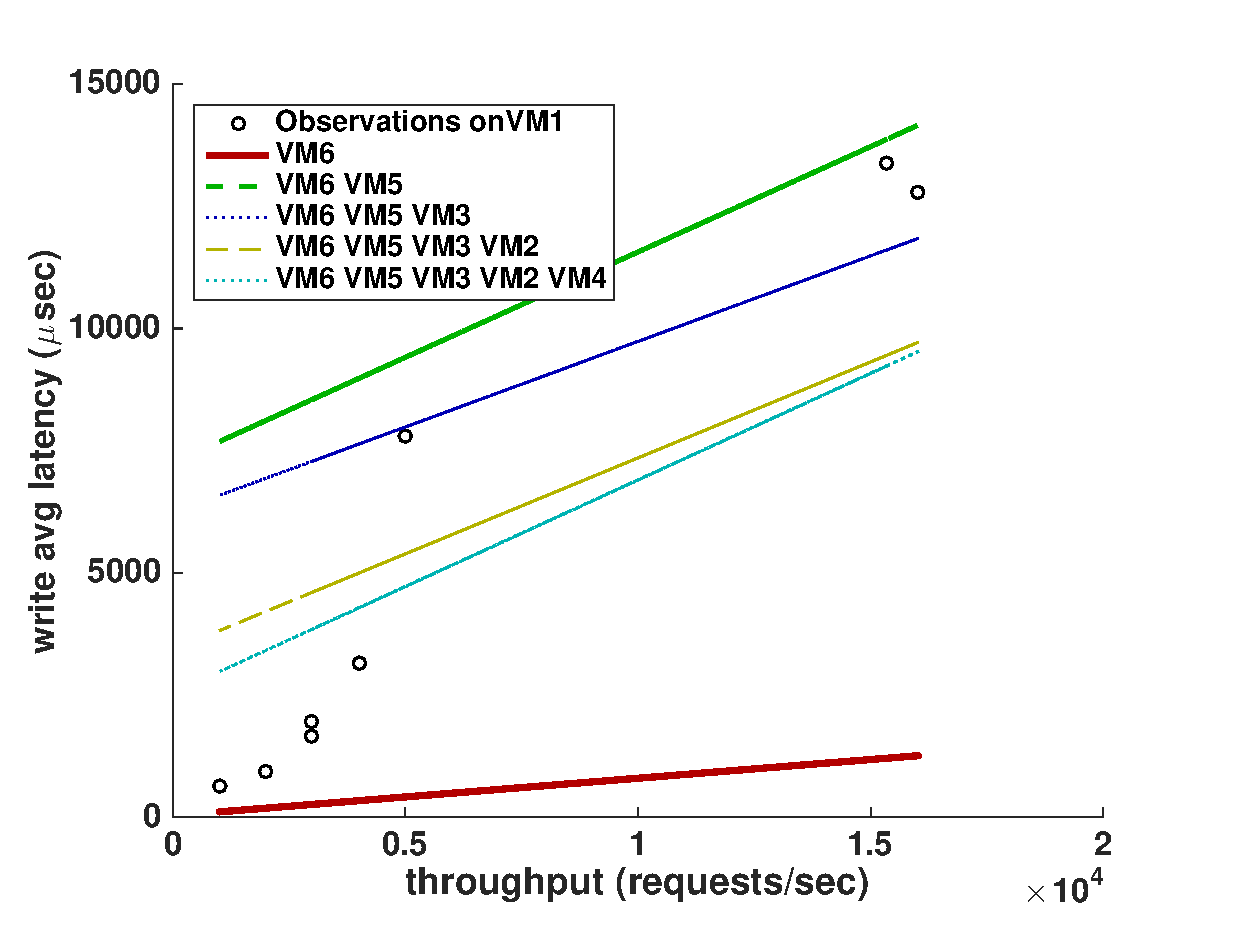
\includegraphics[scale = 0.25]{cassandra_fit_write_avg_latency_r3_2x_r3_x_m3_2x_m3_x_r3__m3_.eps}
    \caption{Cassandra average write latency vs throughput}
    \label{figure:redisbarread}
  \end{figure}
\end{comment}

\begin{figure*}[t]
\subfloat[fig 1]{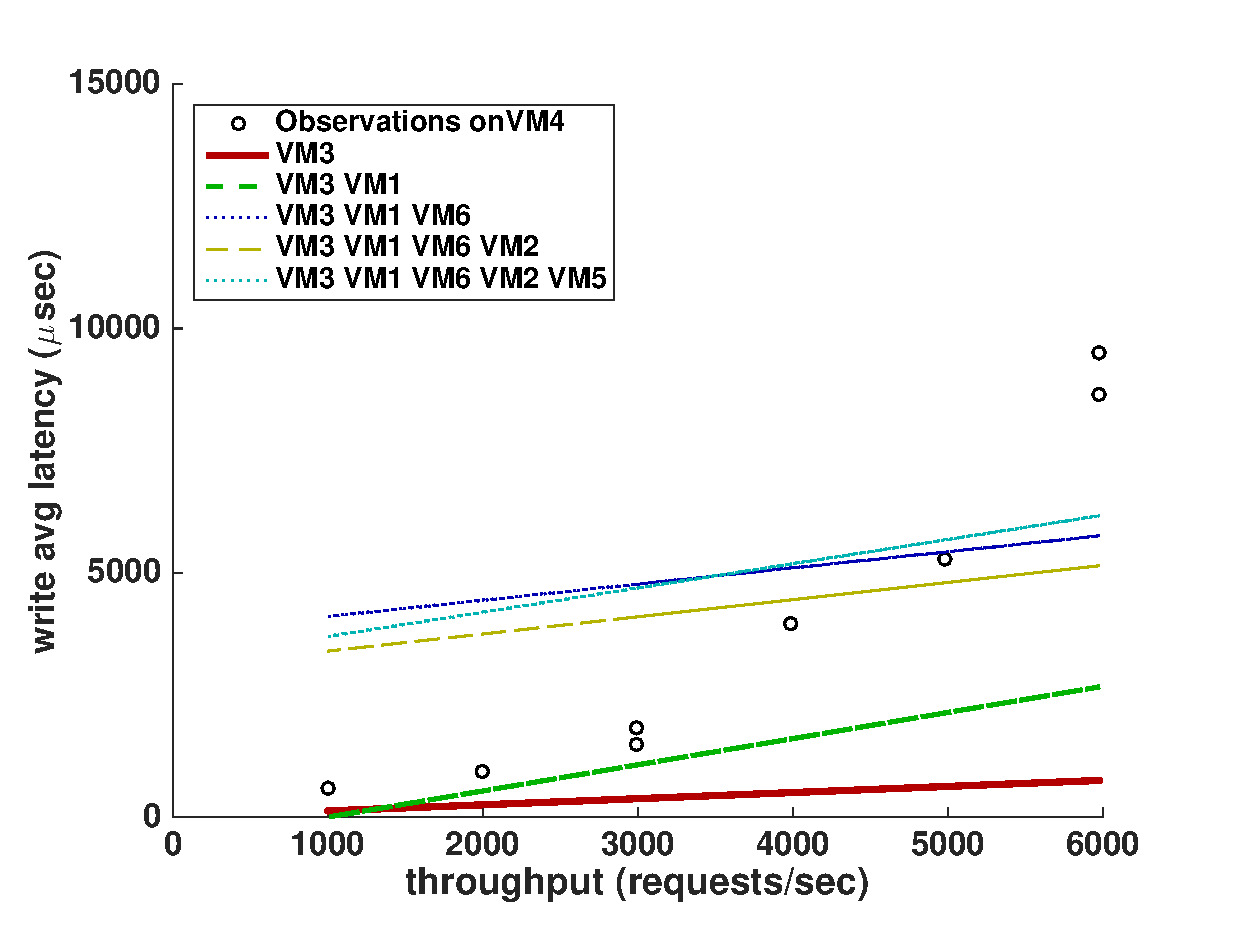
\includegraphics[width=0.5\textwidth]{cassandra_fit_write_avg_latency_m3_2x_m3__r3_2x_m3_x_r3_x_r3_.eps}} 
\subfloat[fig 2]{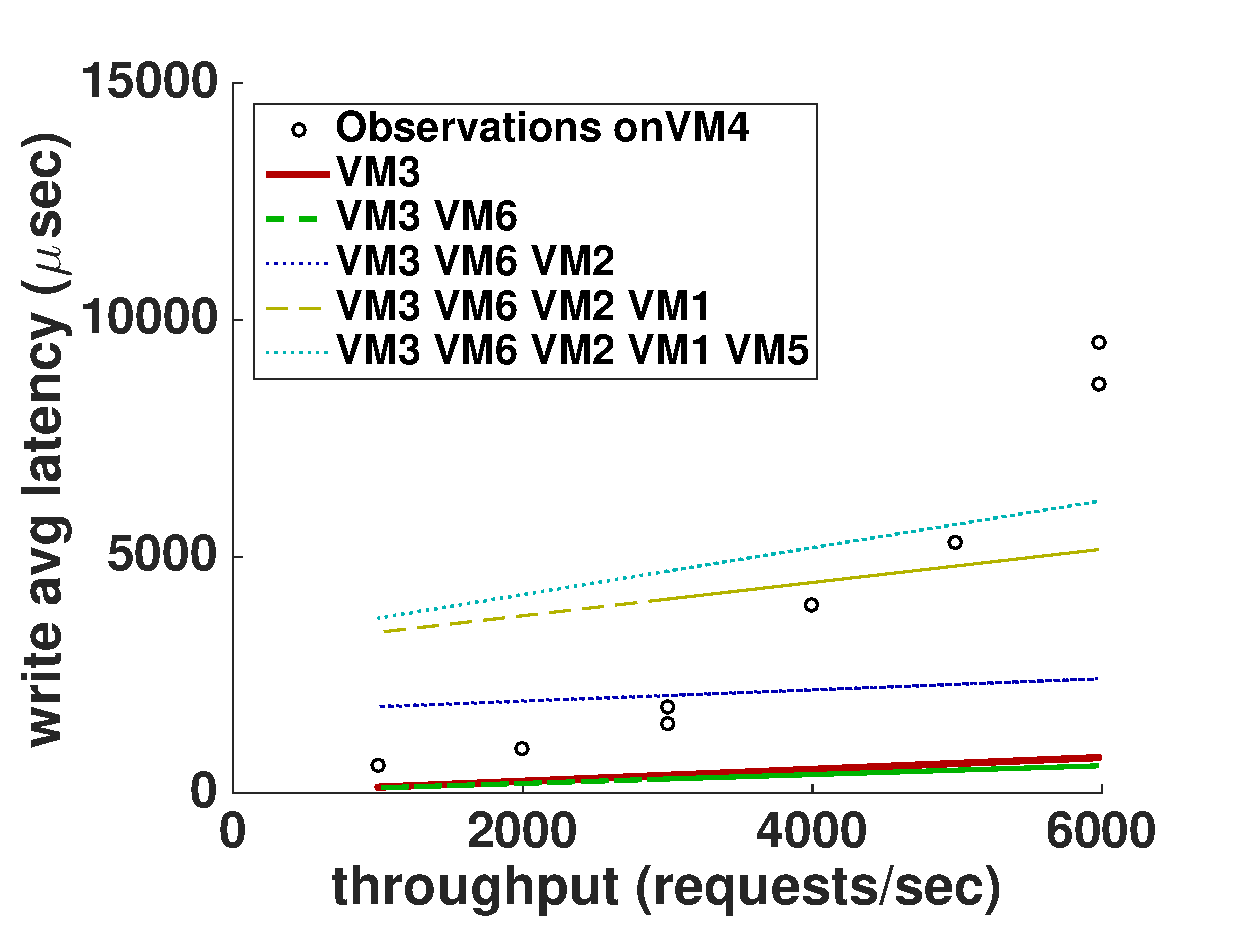
\includegraphics[width=0.5\textwidth]{cassandra_fit_write_avg_latency_m3_2x_r3_2x_m3_x_m3__r3_x_r3_.eps}}\\
\subfloat[fig 3]{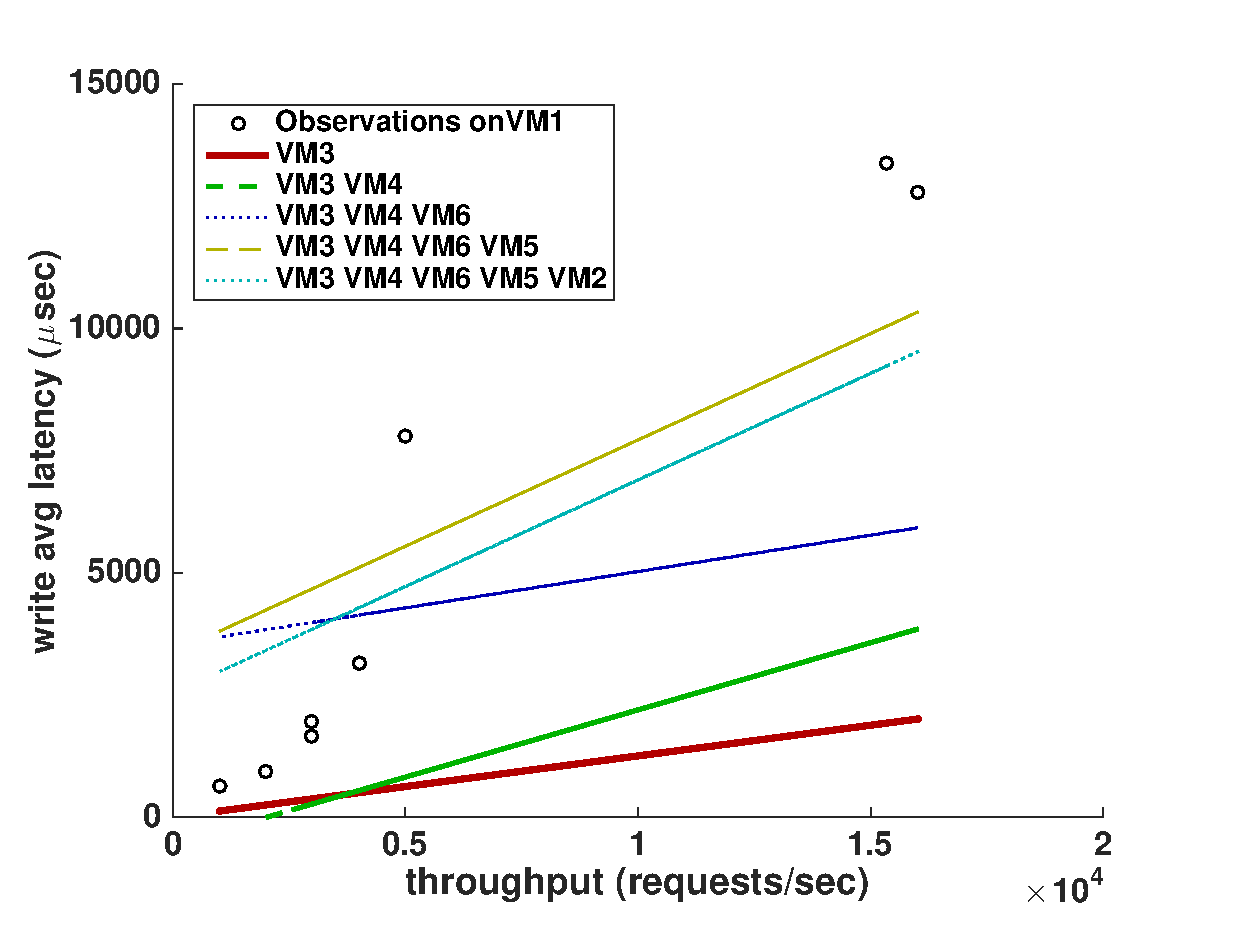
\includegraphics[width=0.5\textwidth]{cassandra_fit_write_avg_latency_m3_2x_r3__r3_2x_r3_x_m3_x_m3_.eps}}
\subfloat[fig 4]{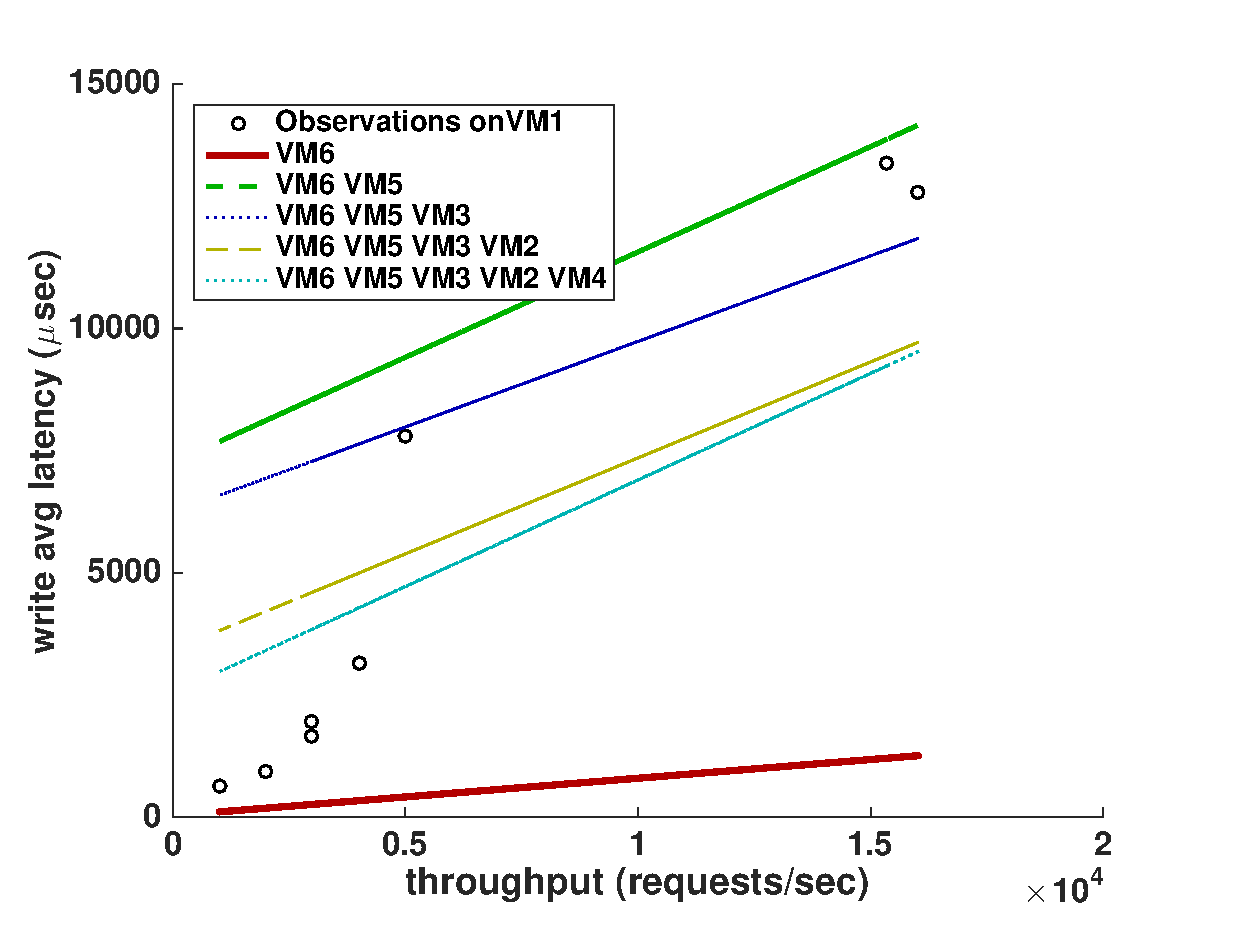
\includegraphics[width=0.5\textwidth]{cassandra_fit_write_avg_latency_r3_2x_r3_x_m3_2x_m3_x_r3__m3_.eps}} 
\caption{Incremental fit for Cassandra Average Write Latency }
\label{some example}
\end{figure*}

% \subsubsection{Evaluation for a Weak Consistency Configuration}

% consistency=ONE

% Workload B (95/5 r/w) with uniform distribution

% Present data for
% 3 VM types: gen,mem,cpu, throughputs 5000-20000, replication factor 3, 5 nodes
